\setcounter{page}{2}
\section{Задание для тренировки}

В лист ресурсов проекта, подготовленного в первой лабораторной работе, был добавлен трудовой ресурс <<Работник>> со стандартной ставкой 120 рублей в день и значением максимума единиц 1100\%, так как к реализации проекта привлекалось не более 11 работников.
Также был добавлен ресурс <<Оборудование>>, который арендуется по ставке 5000 рублей в неделю и на установку и наладку которого было выделено 2000 рублей.
Лист оборудования приведен на рисунке~\ref{fig:test_list}.

\begin{figure}[H]
	\centering
	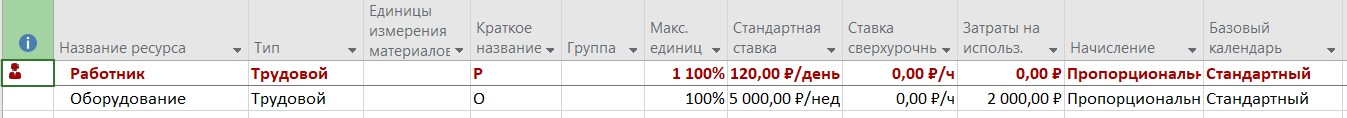
\includegraphics[width=0.9\textwidth]{img/test/equipment.jpg}
	\caption{Лист ресурсов тренировочного проекта}
	\label{fig:test_list}
\end{figure}

Так как ресурс <<Оборудование>> будет использоваться с третьего дня работы B, то необходимо установить задержку в 2 дня.
Данное действие представлено на рисунке~\ref{fig:test_delay}.

\begin{figure}[H]
	\centering
	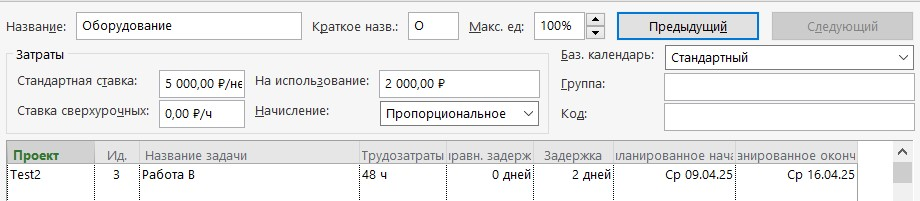
\includegraphics[width=0.9\textwidth]{img/test/delay.jpg}
	\caption{Настройка ресурса <<Оборудование>>}
	\label{fig:test_delay}
\end{figure}

В результате указания распределения ресурсов получена диаграмма Ганта, представленная на рисунке~\ref{fig:test_gant}.
	
\begin{figure}[H]
	\centering
	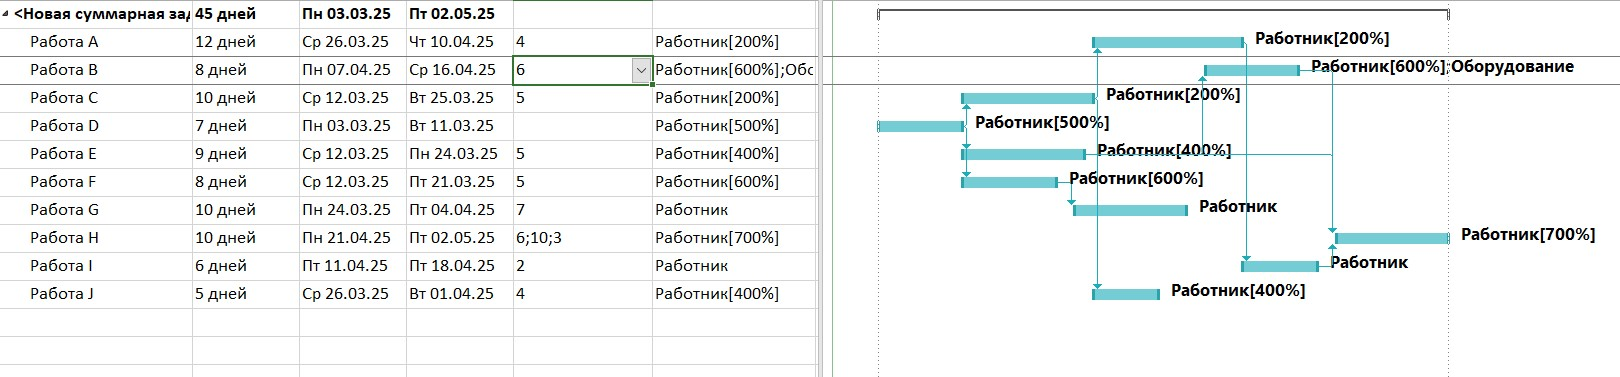
\includegraphics[width=0.9\textwidth]{img/test/add_worker.jpg}
	\caption{Диаграмма Ганта тренировочного проекта}
	\label{fig:test_gant}
\end{figure}

Полученные для ресурса <<Работник>> перегрузки демонстрируются на рисунке~\ref{fig:test_overflow}.
	
\begin{figure}[H]
	\centering
	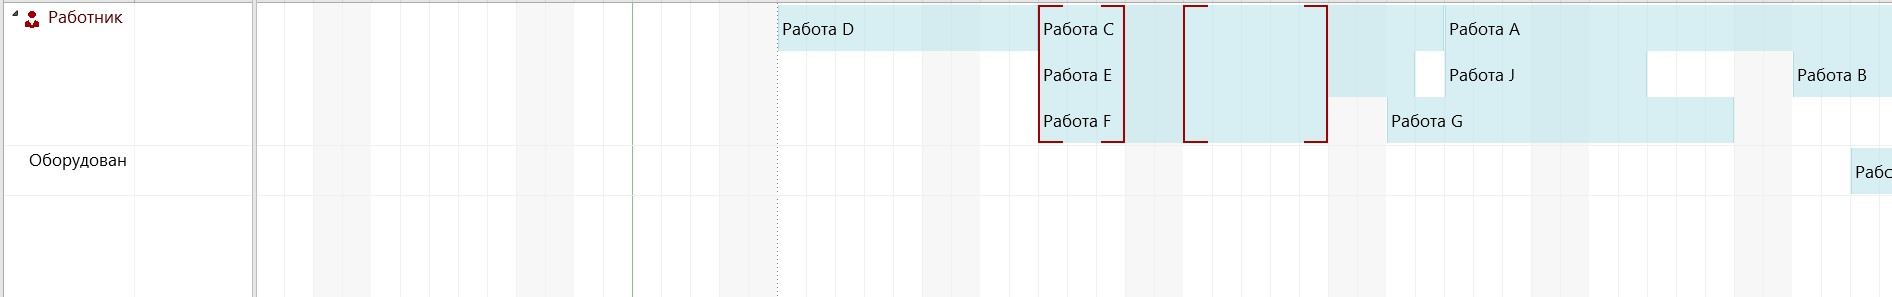
\includegraphics[width=0.9\textwidth]{img/test/overflow.jpg}
	\caption{Демонстрация перегрузки ресурса <<Работник>>}
	\label{fig:test_overflow}
\end{figure}

Перегрузка ресурса <<Работник>> возникает из-за его одновременного задействования в работах C, E и F.

На рисунке~\ref{fig:test_final} представлены затраты на проект.

\begin{figure}[H]
	\centering
	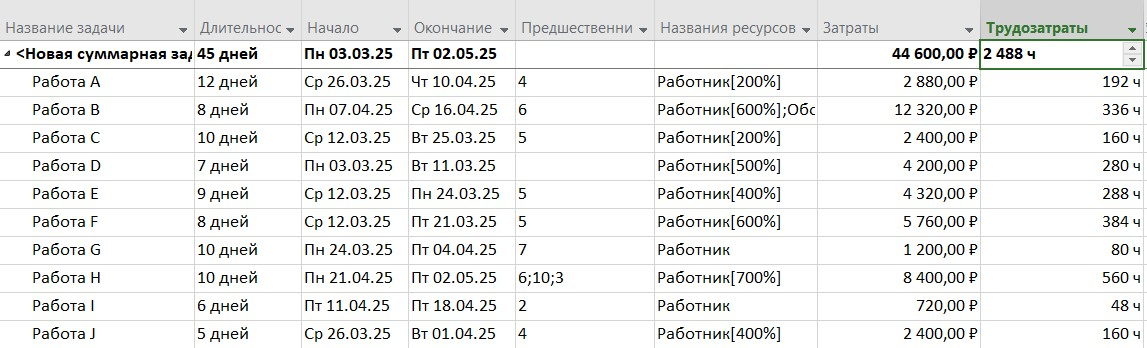
\includegraphics[width=0.9\textwidth]{img/test/final.jpg}
	\caption{Затраты на тренировочный проект}
	\label{fig:test_final}
\end{figure}

Затраты на работников составили 36600 рублей, а затраты на оборудование~---~8000 рублей.
Бюджет тренировочного проекта составил 44600 рублей.

\section{Задание №1}

Проект представляет собой создание карты города.
В проекте участвуют 16 разработчиков, бюджет проекта~---~50000 рублей, длительность проекта~---~6 месяцев.
Дата начала проекта~---~первый рабочий день марта текущего года.

Лист ресурсов проекта представлен на рисунке~\ref{fig:list}.

\begin{figure}[H]
	\centering
	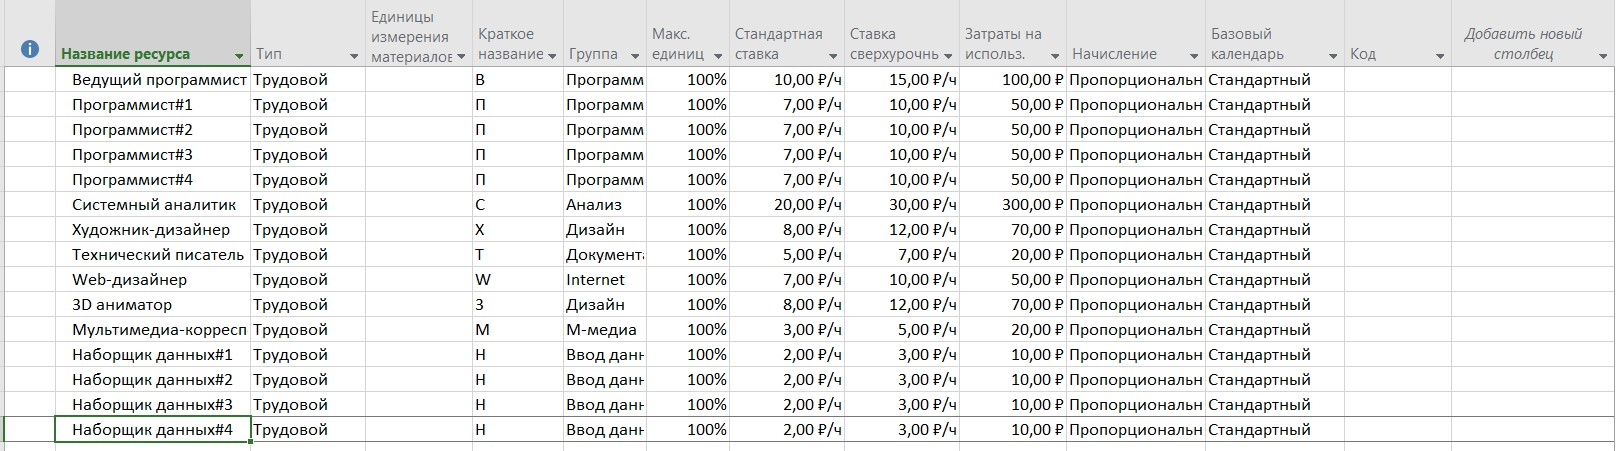
\includegraphics[width=0.9\textwidth]{img/task1/list.jpg}
	\caption{Лист ресурсов проекта}
	\label{fig:list}
\end{figure}

\section{Задание №2}

На рисунке~\ref{fig:gant} приведена диаграмма Ганта после назначения задачам ресурсов.

\begin{figure}[H]
	\centering
	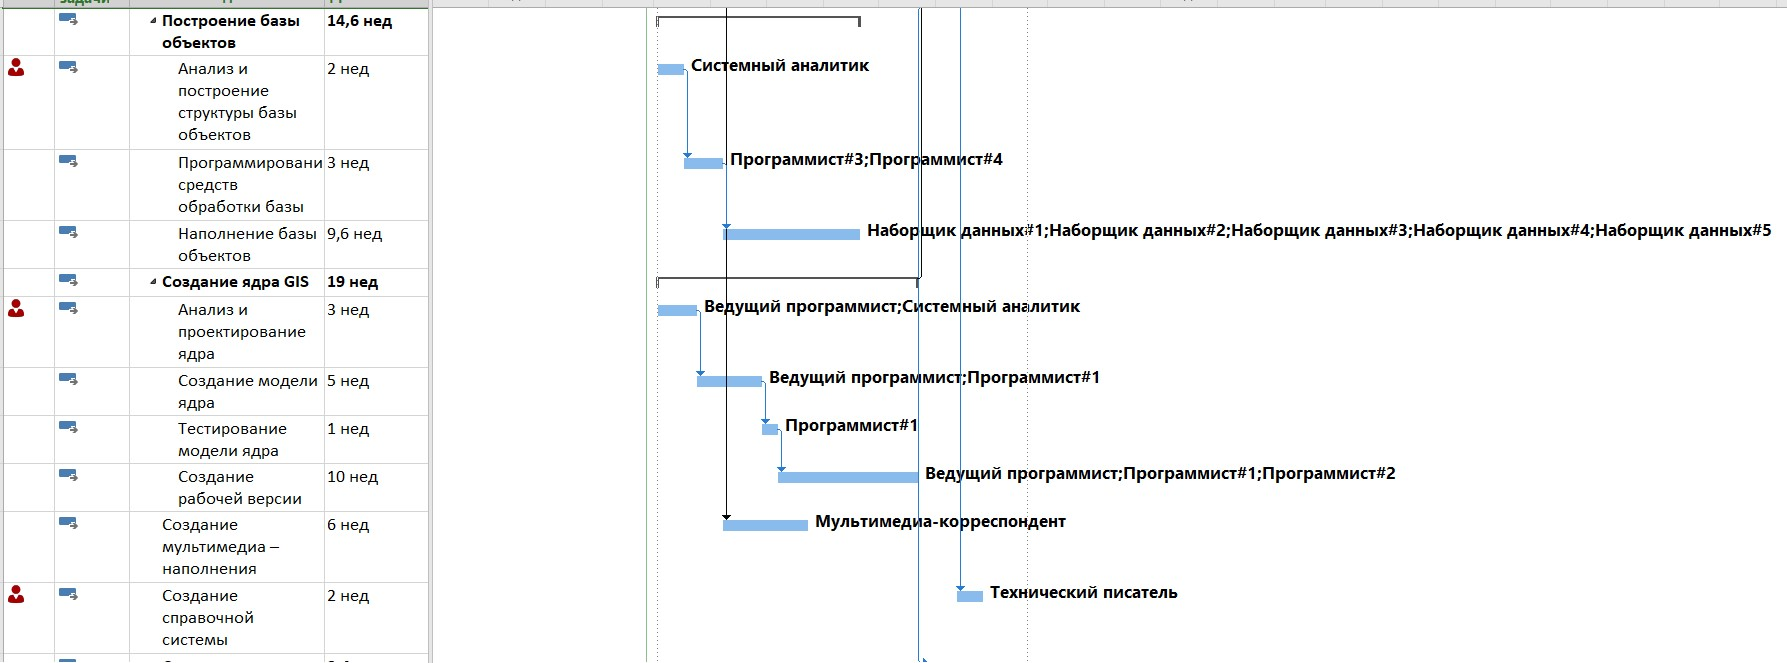
\includegraphics[width=0.9\textwidth]{img/task2/gant.jpg}
	\caption{Диаграмма Ганта после назначения ресурсов задачам проекта}
	\label{fig:gant}
\end{figure}

Как видно по диаграмме Ганта и листу ресурсов, приведенном на рисунке~\ref{fig:list_overflow}, ресурсы <<Системный аналитик>>, <<Художник-дизайнер>> и <Технический писатель>> перегружены.

\begin{figure}[H]
	\centering
	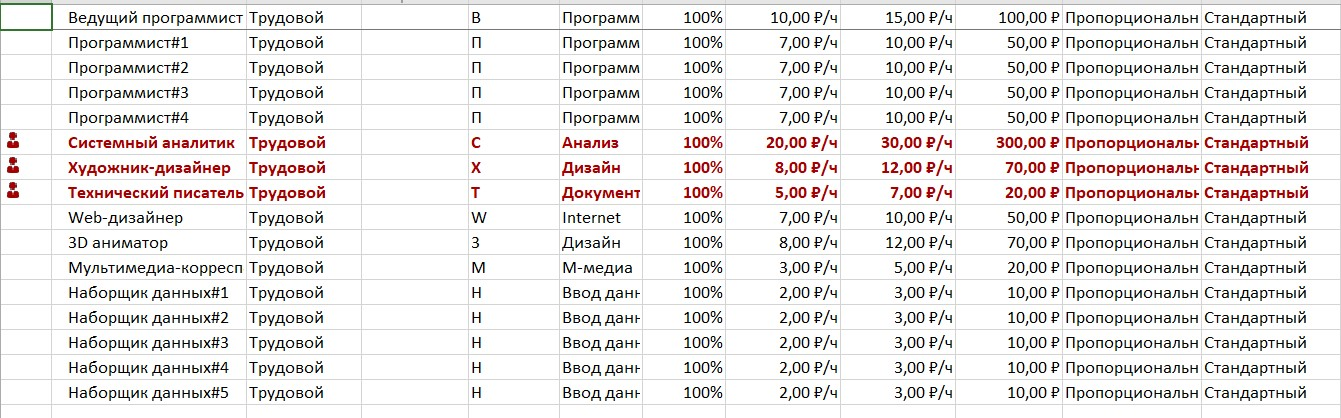
\includegraphics[width=0.9\textwidth]{img/task2/list.jpg}
	\caption{Лист ресурсов с указанием перегруженных ресурсов}
	\label{fig:list_overflow}
\end{figure}

Появление перегрузки для ресурса <<Системный аналитик>> связано с тем, что данный ресурс задействован при выполнении задач <<Анализ и построение структуры базы объектов>> и <<Анализ и проектирование ядра>>, сроки реализаций которых накладываются.

Появление перегрузки для ресурса <<Художник-дизайнер>> связано с тем, что данный ресурс задействован при выполнении задач <<Разработка дизайна руководства>> и <<Разработка дизайна сайта>>, сроки реализаций которых накладываются.

Появление перегрузки для ресурса <<Технический писатель>> связано с тем, что данный ресурс задействован при выполнении задач <<Написание руководства пользователя>> и <<Создание справочной системы>>, сроки реализаций которых накладываются.

Назначение фиксированных затрат в размере 1000 рублей на задачи 2, 8 и 12 приведено на рисунке~\ref{fig:cost}.

\begin{figure}[H]
	\centering
	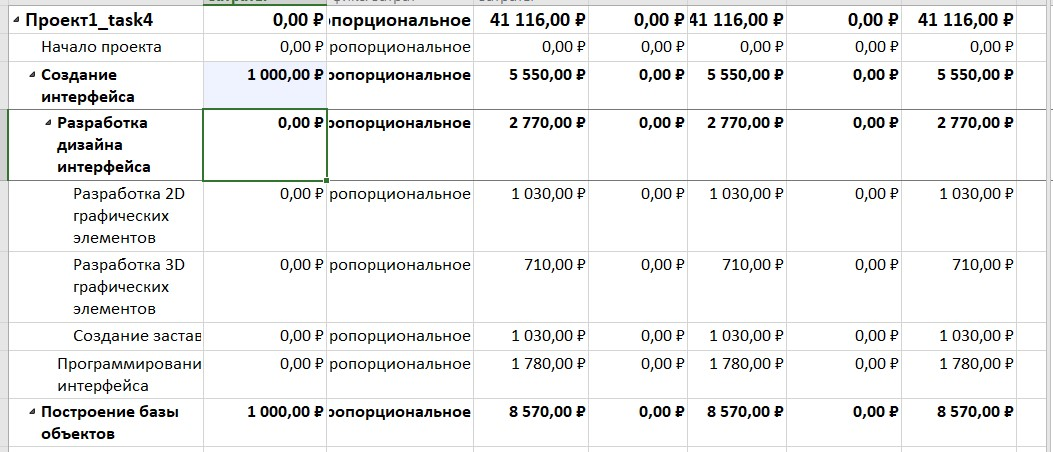
\includegraphics[width=0.9\textwidth]{img/task2/cost.jpg}
	\caption{Назначение фиксированных затрат}
	\label{fig:cost}
\end{figure}

Добавление ресурса <<Сервер>> приведено на рисунках~\ref{fig:server} и~\ref{fig:gant_server}.

\begin{figure}[H]
	\centering
	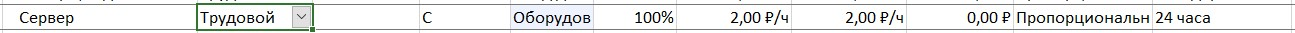
\includegraphics[width=0.9\textwidth]{img/task2/server.jpg}
	\caption{Добавление ресурса <<Сервер>> в лист ресурсов}
	\label{fig:server}
\end{figure}

\begin{figure}[H]
	\centering
	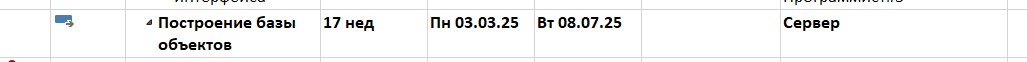
\includegraphics[width=0.9\textwidth]{img/task2/gant_server.jpg}
	\caption{Добавление ресурса <<Сервер>> для задачи <<Построение базы объектов>>}
	\label{fig:gant_server}
\end{figure}

Сервер используется 24 часа в сутки, поэтому необходимо изменить базовый календарь на <<24 часа>>.
Так как затраты на сервер зависят от количества часов работы, он является трудовым ресурсом.

\section{Задание №3}

Структуризация затрат и трудозатрат по группам ресурсов и их графическое представление приведены на рисунках~\ref{fig:group}~---~\ref{fig:work_diagram}.

\begin{figure}[H]
	\centering
	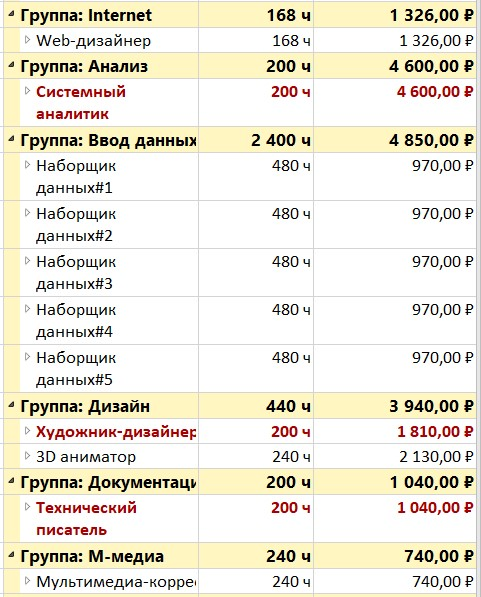
\includegraphics[width=0.9\textwidth]{img/task3/group.jpg}
	\caption{Структуризация затрат по группам ресурсов}
	\label{fig:group}
\end{figure}

\begin{figure}[H]
	\centering
	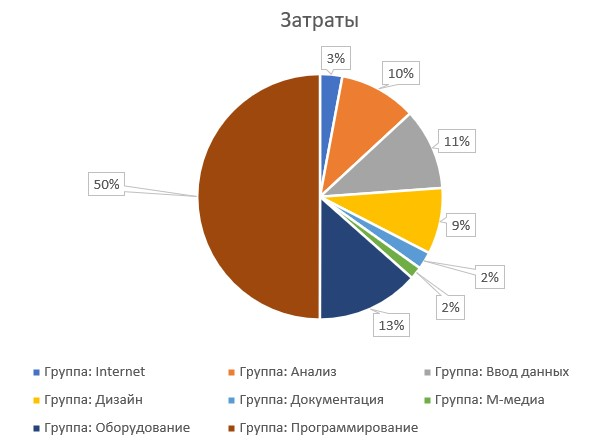
\includegraphics[width=0.9\textwidth]{img/task3/diagram.jpg}
	\caption{Графическое представление структуризации затрат по группам ресурсов}
	\label{fig:graphic_group}
\end{figure}

\begin{figure}[H]
	\centering
	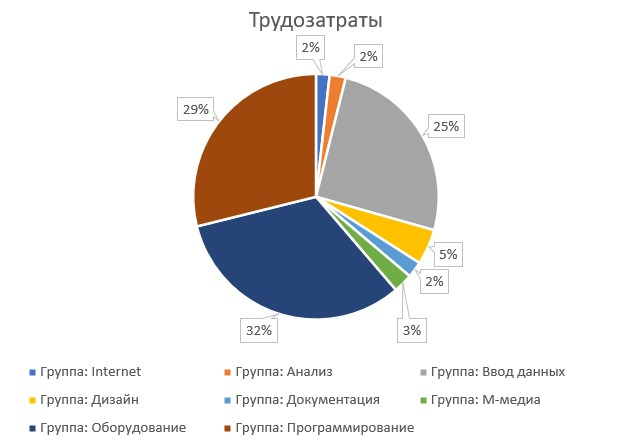
\includegraphics[width=0.9\textwidth]{img/task3/work_diagram.jpg}
	\caption{Графическое представление структуризации трудозатрат по группам ресурсов}
	\label{fig:work_diagram}
\end{figure}

Таким образом, самыми затратными ресурсами являются ресурсы группы <<Программирование>> (22580 рублей, 2720 часов) и <<Сервер>> (6102 рубля, 3051 час).
Затраты на программистов объясняются высокой квалификацией работников.
Их трудозатраты соотносятся с законом Брукса, то есть занимают 30\% времени работы.
Стоит задуматься о приобретении сервера вместо его аренды.
Группа <<Ввод данных>> (4850 рублей, 2400 часов) вносит существенный вклад в трудозатраты при сравнительно небольших затратах на ресурс.
Таким образом, можно для ускорения их работы нанять еще несколько наборщиков, так как это не сильно повлияет на затраты.
На аналитика тратится размер бюджета, несоразмерный объему работы, то есть распределение его времени работы на проекте необходимо оптимизировать.
Наименьший вклад в затраты и трудозатраты вносят ресурсы групп <<Internet>>, <<M-медиа>> и <<Документация>>.

Итоговые затраты и трудозатраты на проект приведены на рисунке~\ref{fig:final}.
\begin{figure}[H]
	\centering
	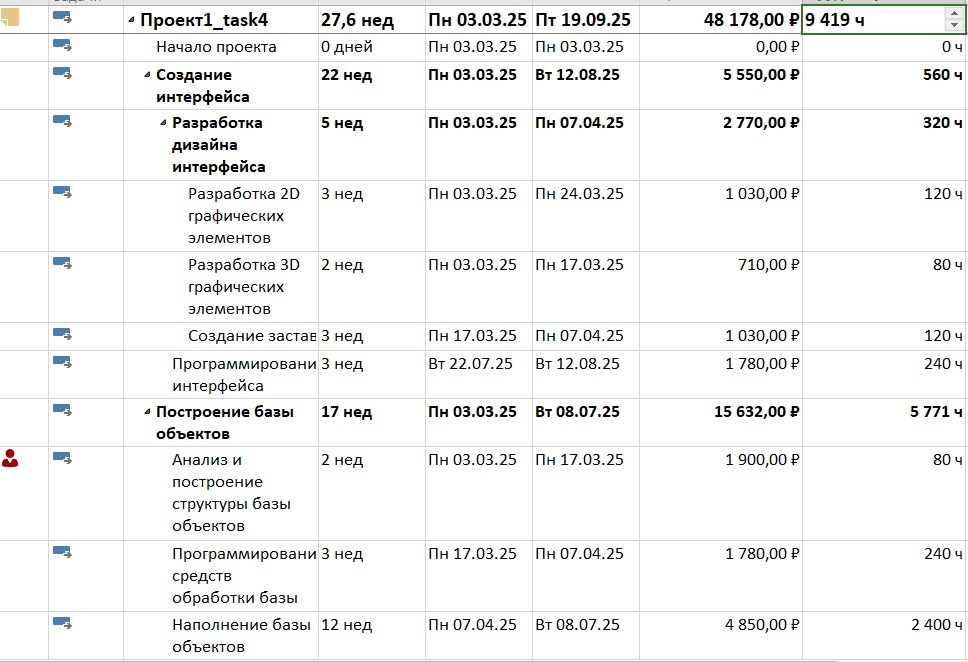
\includegraphics[width=0.9\textwidth]{img/task3/final.jpg}
	\caption{Указание затрат и трудозатрат на проект}
	\label{fig:final}
\end{figure}

Таким образом, на проект требуется 48178 рублей, что укладывается в бюджет размером 50000 рублей.

\begin{comment}
Датой начала проекта является первый рабочий день марта текущего года.
Настройка даты начала проекта представлена на рисунке~\ref{fig:proj_start}.

\begin{figure}[H]
	\centering
	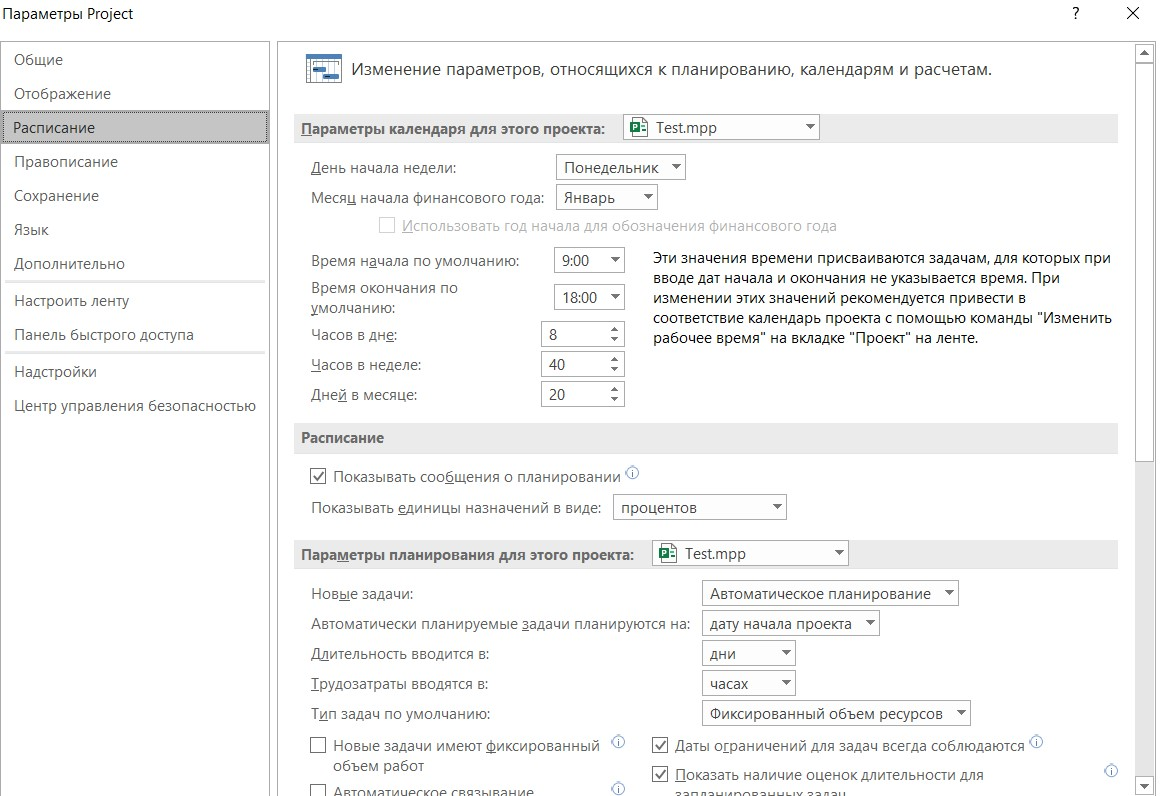
\includegraphics[width=0.9\textwidth]{img/test/params.jpg}
	\caption{Настройка даты начала проекта}
	\label{fig:proj_start}
\end{figure}

Временные характеристики проекта приведены в таблице~\ref{tbl:compare}.

\begin{table}[ht]
	\small
	\begin{center}
		\begin{threeparttable}
			\caption{Временные характеристики проекта}
			\label{tbl:compare}
			\begin{tabular}{|c|c|}
				\hline
				\textbf{Название работы}                                                & \textbf{\begin{tabular}[c]{@{}c@{}}Длительность (дни)\end{tabular}} \\ \hline
				\begin{tabular}[c]{@{}c@{}}Работа A\end{tabular}  & 12 \\ \hline
				\begin{tabular}[c]{@{}c@{}}Работа B\end{tabular}  & 6 \\ \hline
				\begin{tabular}[c]{@{}c@{}}Работа C\end{tabular}  & 10 \\ \hline
				\begin{tabular}[c]{@{}c@{}}Работа D\end{tabular}  & 7 \\ \hline
				\begin{tabular}[c]{@{}c@{}}Работа E\end{tabular}  & 9 \\ \hline
				\begin{tabular}[c]{@{}c@{}}Работа F\end{tabular}  & 8 \\ \hline
				\begin{tabular}[c]{@{}c@{}}Работа G\end{tabular}  & 10 \\ \hline
				\begin{tabular}[c]{@{}c@{}}Работа H\end{tabular}  & 10 \\ \hline
				\begin{tabular}[c]{@{}c@{}}Работа I\end{tabular}  & 6 \\ \hline
				\begin{tabular}[c]{@{}c@{}}Работа J\end{tabular}  & 5 \\ \hline
			\end{tabular}
		\end{threeparttable}
	\end{center}
\end{table}

На рисунке~\ref{fig:test} приведена построенная диаграмма Ганта.

\begin{figure}[H]
	\centering
	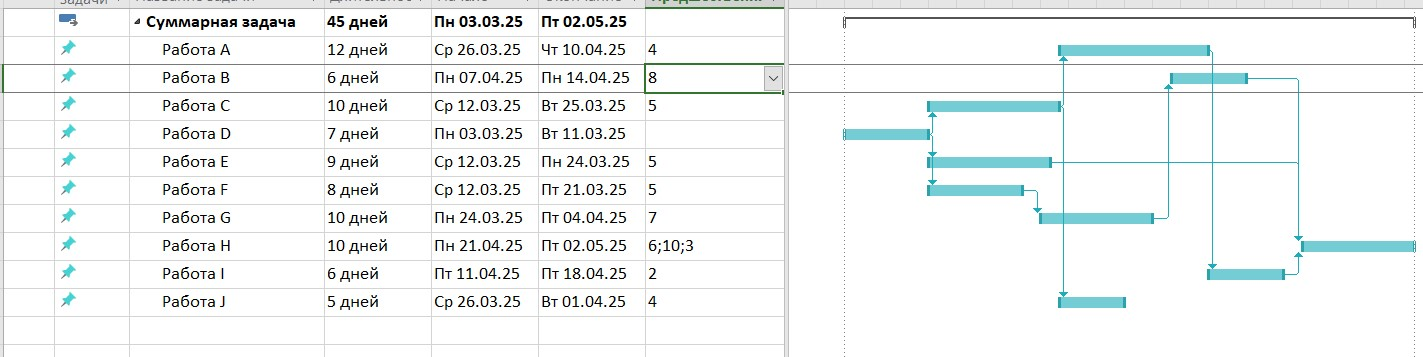
\includegraphics[width=0.9\textwidth]{img/test/test.jpg}
	\caption{Демонстрация выполнения задания для тренировки}
	\label{fig:test}
\end{figure}

Таким образом, определено, что длительность проекта для тренировки составляет 45 дней, дата его завершения~---~02.05.2025.

\section{Задание №1}

Проект представляет собой создание карты города.
В проекте участвуют 16 разработчиков, бюджет проекта~---~50000 рублей, длительность проекта~---~6 месяцев.
Дата начала проекта~---~первый рабочий день марта текущего года.

Перед добавлением задач необходимо настроить параметры проекта, находящиеся во вкладке $\text{Файл} \rightarrow \text{Параметры} \rightarrow \text{Расписание}$.
Настройка параметров представлена на рисунке~\ref{fig:parameters}.

\begin{figure}[H]
	\centering
	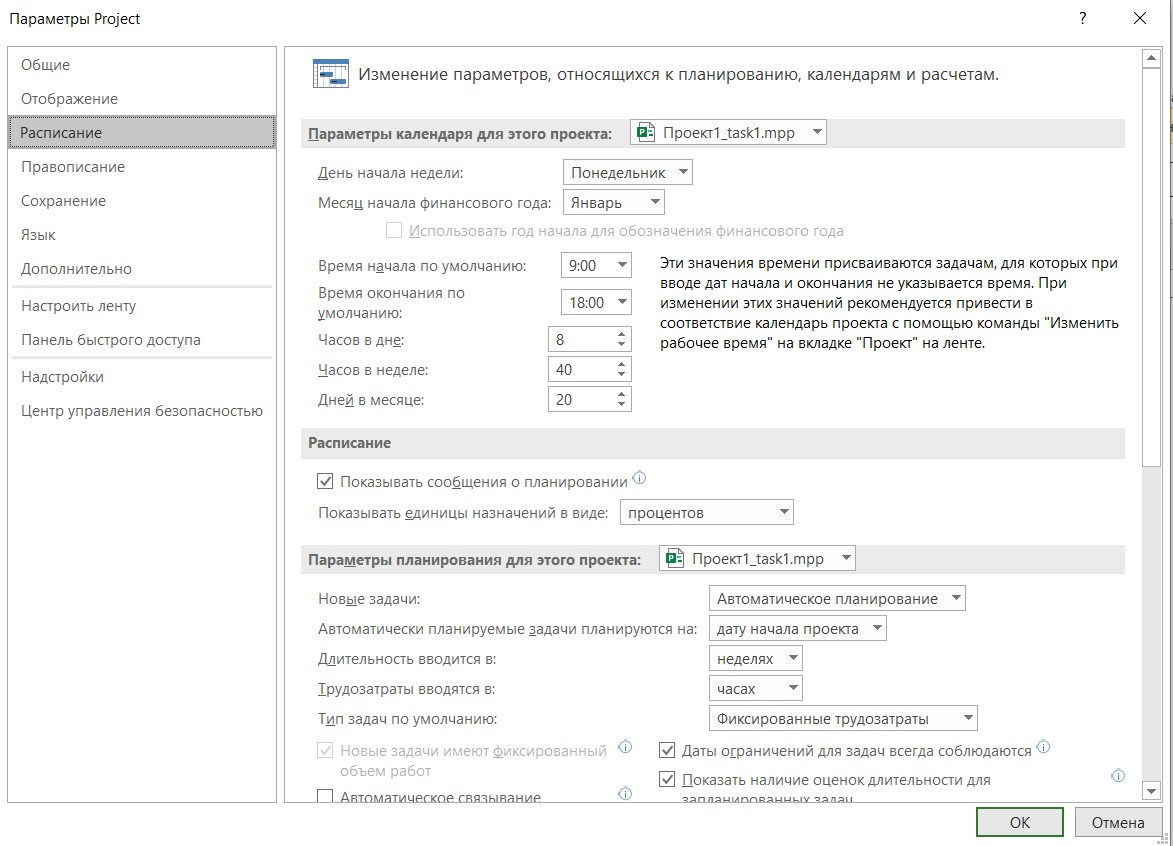
\includegraphics[width=0.9\textwidth]{img/task1/parameters.jpg}
	\caption{Настройка параметров проекта}
	\label{fig:parameters}
\end{figure}

Также необходимо внести в календарь праздничные дни и предшествующие им дни с укороченным рабочим графиком.
Для планируемого проекта такими днями являются майские праздники, день России в июне и день народного единства в ноябре.
Настройка календаря проекта приведена на рисунке~\ref{fig:calendar}.

\begin{figure}[H]
	\centering
	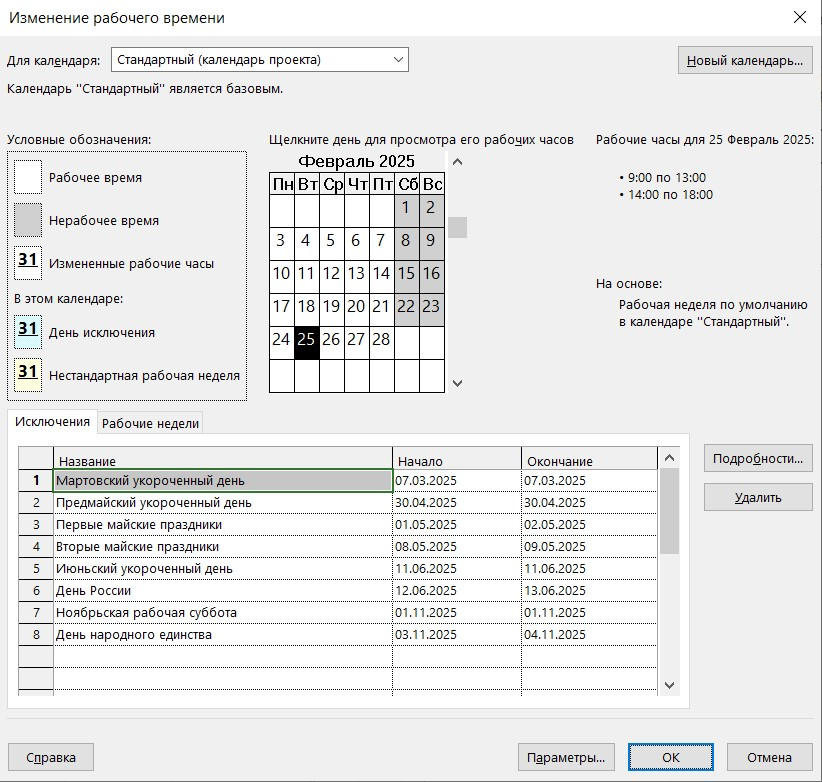
\includegraphics[width=0.9\textwidth]{img/task1/calendar.jpg}
	\caption{Настройка календаря проекта}
	\label{fig:calendar}
\end{figure}

Информацию о проекте можно посмотреть в Заметках, приведенных на рисунке~\ref{fig:notes}.

\begin{figure}[H]
	\centering
	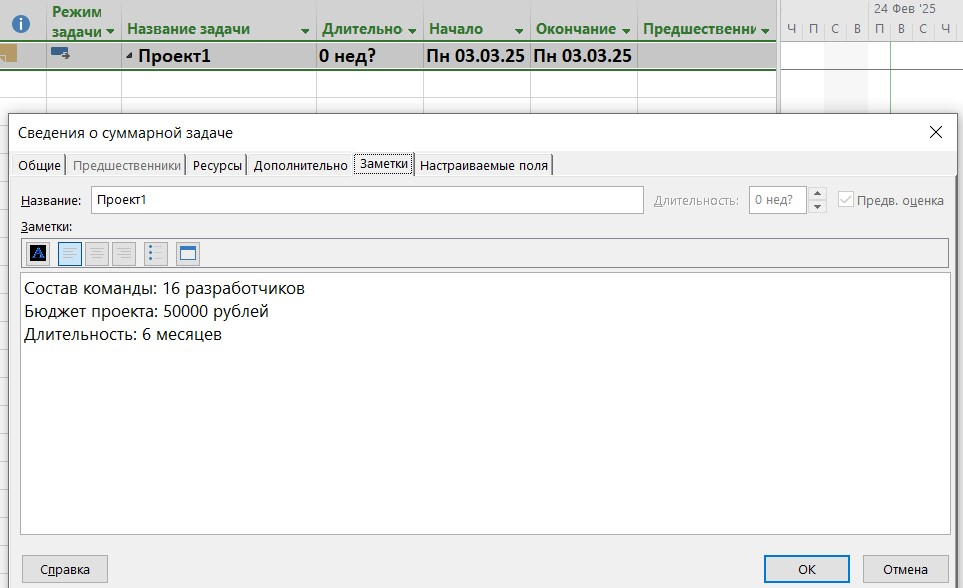
\includegraphics[width=0.9\textwidth]{img/task1/notes.jpg}
	\caption{Заметки проекта}
	\label{fig:notes}
\end{figure}

\section{Задание №2}

После настройки параметров проекта необходимо добавить задачи.
Так как в настройках указано, что автоматически планируемые задачи планируются на дату начала проекта, все задачи начинаются с третьего марта, что видно по диаграмме Ганта и столбцу <<Начало>> на рисунке~\ref{fig:task2}.

\begin{figure}[H]
	\centering
	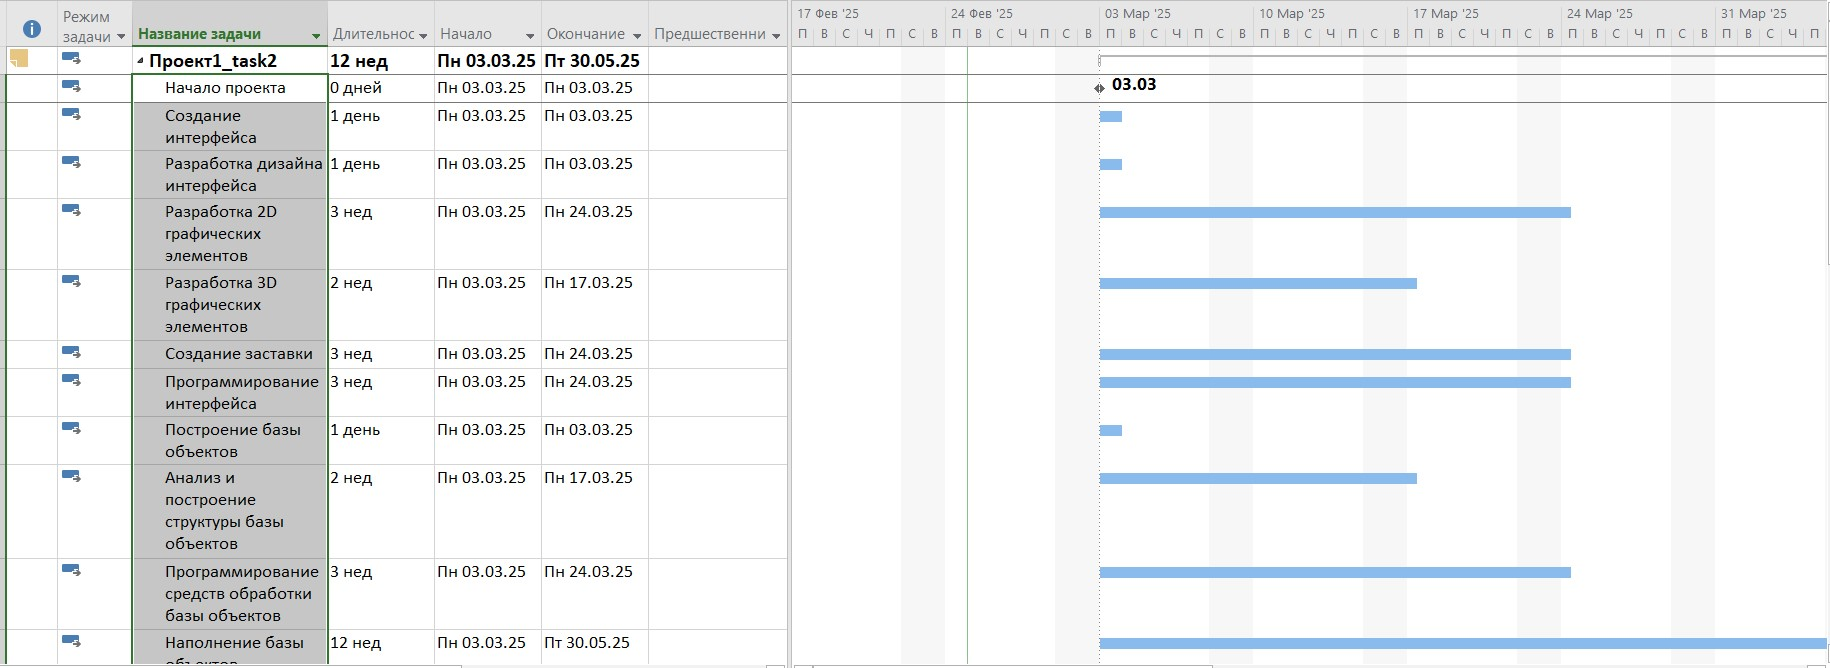
\includegraphics[width=0.9\textwidth]{img/task2/tasks.jpg}
	\caption{Диаграмма Ганта}
	\label{fig:task2}
\end{figure}

\section{Задание №3}

При проведении структурирования списка задач были выделены фазы проекта.
Результат структурирования списка задач приведен на рисунке~\ref{fig:task3}.

\begin{figure}[H]
	\centering
	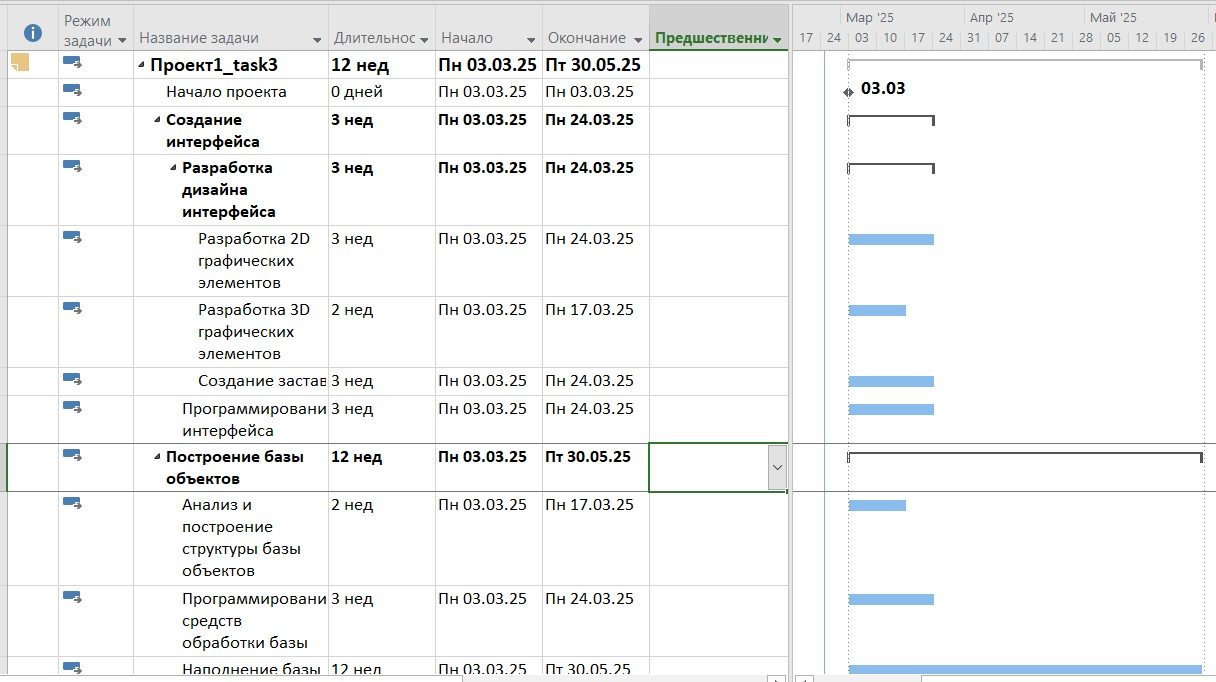
\includegraphics[width=0.9\textwidth]{img/task3/task3.jpg}
	\caption{Диаграмма Ганта после структурирования списка задач}
	\label{fig:task3}
\end{figure}

\section{Задание №4}

После структурирования списка задач необходимо указать связи между ними. 
Предшествующие задачи можно указать в столбце <<Предшественники>>.
По умолчанию устанавливается тип связи Окончание~---~Начало, при котором последующая задача начинается после окончания предыдущей.
В случае необходимости выбора другого типа связи необходимо дважды кликнуть по связи между задачами на диаграмме Ганта.
В появившемся модальном окне можно выбрать тип связи, а также указать время опережения/запаздывания.

Результат настройки связей между задачами приведен на рисунках~\ref{fig:task41} и~\ref{fig:task42}.

\begin{figure}[H]
	\centering
	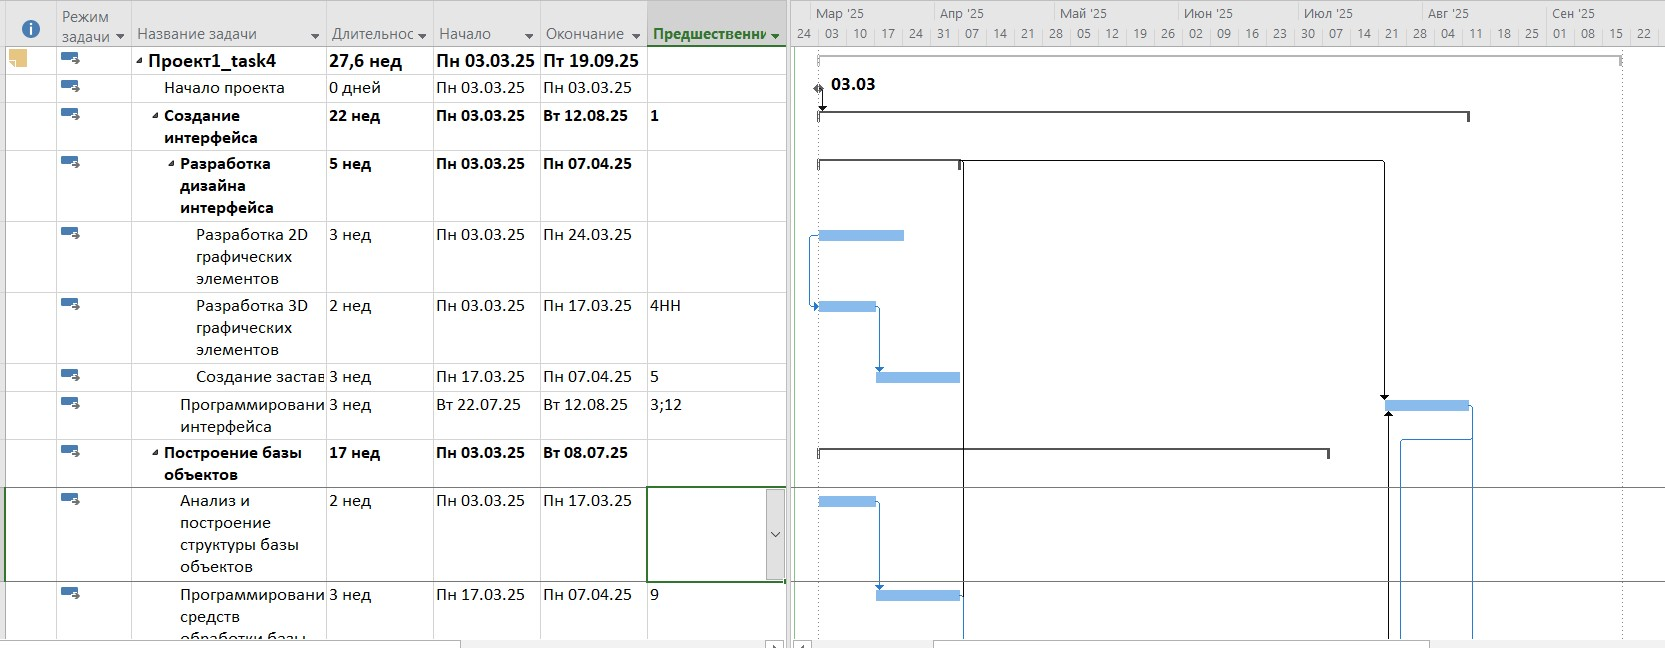
\includegraphics[width=0.9\textwidth]{img/task4/task4.jpg}
	\caption{Диаграмма Ганта с датой начала проекта}
	\label{fig:task41}
\end{figure}

\begin{figure}[H]
	\centering
	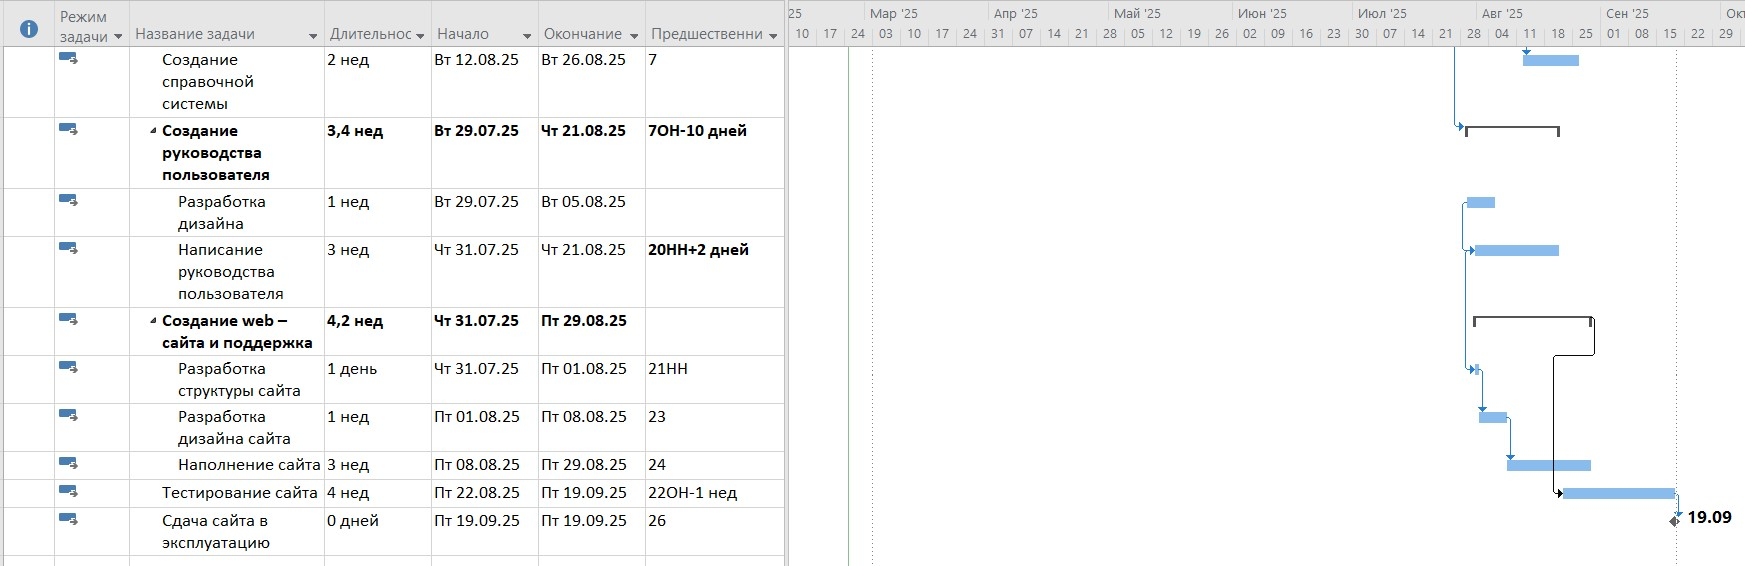
\includegraphics[width=0.9\textwidth]{img/task4/task4_1.jpg}
	\caption{Диаграмма Ганта с датой завершения проекта}
	\label{fig:task42}
\end{figure}

В результате планирования проекта было определена дата завершения проекта: 19 сентября 2025 года.
\end{comment}